\chapter{MEC Neurons Encode Subsets of Navigational Variables}
\label{chapterlabel5}
After the discovery of grid cells in MEC, an explosion of literature on MEC cell characterisation shows that rat MEC contains grid cells, speed cells, head direction cells, boundary vecotr cells, conjugative cells, etc. In addition, rat MEC cells can have multiplexed and heterogeneous codes and this finding applies a multivariate generalised linear model to find tunings for speed, 2D space, head direction, theta phase together. However, mice are found to have 0-10\% grid cell yield and the representation can drift over time. Further to that, most mice MEC research focused on VR studies to make advantage of this tool with high yield recording devices. This approach, including this thesis, restrains the spatial tuning to be one-dimensional and focuses on partial functions of MEC. For example, focuses on cue-tuning, focuses on distance-tuning, tried to identify grid cells with spatial spectrogram and how they evolve in more visually-dominated environments. These selective approaches provide many insights on MEC's role in mutiple contexts and how diverse MEC can be. However, there still lacks a comprehensive characterisation of MEC cells' roles together in VR setting. In this chapter, by the advantage of using visually-complex environments in this thesis, a similar multiplexed and heterogeneous population code is found in mouse MEC with some deviations from previous findings. 

\section{Method}
\subsection{Spatial Tuning}
Cells with 95\% peak percentile from shuffled data in the two tracks, > 0.1Hz mean firing rate in the tracks and median variance > 0.6 across 10 folds of all laps (removes neurons only fire in some random laps). Spikes are first smoothed with 200 ms gaussian window in time at 60 Hz and binned at 2 cm bins. The spatial bins are extended to final position where the gray screen ends (3-5s after the lap finishes at 140 cm) to trace the post-VR dynamics.

\subsection{Speed Tuning}
Speed response is binned at 1 cm/s bin from 0 cm/s to 40 cm/s. A skewed gaussian line fitting is applied to binned speed response from (citation):
equation

The skewed peak is defined as which speed the neuron prefers, which is divided into untuned (\(R^2 < 0.15\)), low-pass, band-pass (5, 10, 15, 20, 25, 30), and high-pass.

\subsection{Generalised Linear Model}
\subsubsection{Model Structure}
A Generalized Linear Model (GLM) with a log link function with Poisson distribution is used to connect the spike count to a linear combination of predictors and the log link function makes their relationship multiplicative. The core equation is:

\begin{equation}
\log(\lambda_t) = \eta_t = \mathbf{X}_t \cdot \mathbf{w}
\end{equation}
and the spiking activity of a neuron can be predicted by:
\[\lambda_t = \exp(\mathbf{X}_t \cdot \mathbf{w}) = \exp(w_0) \exp(\mathbf{X}_{t, \text{pos,t1}} \cdot \mathbf{w}_{\text{pos,t1}}) \exp(\mathbf{X}_{t, \text{pos,t2}} \cdot \mathbf{w}_{\text{pos,t2}}) \dots
\]
where:
\begin{itemize}
    \item $\lambda_t$ is the instantaneous spike count at time $t$.
    \item $\eta_t$ is the linear predictor.
    \item $\mathbf{X}_t$ is a row vector representing the values of all predictors at time $t$.
    \item $\mathbf{w}$ is the column vector of weights (coefficients) that the model learns.
\end{itemize}

The full linear predictor, $\eta_t$, is an additive combination of several components:
\begin{equation}
\eta_t = w_0 + \sum_{j=1}^{P} X_{t,j,\text{pos,t1}} \cdot w_{j,t1} + \sum_{j=1}^{P} X_{t,j,\text{pos,t2}} \cdot w_{j,t2} + \sum_{k=1}^{S} X_{t,k,\text{speed}} \cdot w_{k} + \sum_{t=0 s}^{t=0.5 s}X_{t,\text{reward}} \cdot w_{t}
\end{equation}
Each component of the design matrix $\mathbf{X}$ is constructed as follows:


\subsubsection{\textbf{Track-Specific Spatial Predictors ($\mathbf{X}_{\text{pos,t1}}$, $\mathbf{X}_{\text{pos,t2}}$):}}

The track is divided into spatial bins at 5 cm. A binary matrix is created where each column corresponds to a bin, and the value is 1 if the animal is in that bin at that time.
This binary matrix is multiplied element-wise by a mask for the corresponding track. This ensures the predictors are zero when the animal is on the other track.
Finally, each column of the resulting matrix is smoothed over time with a 1D Gaussian filter to create a more biologically plausible, graded representation of the animal's presence in each bin.
 
\subsubsection{\textbf{Speed Predictor ($\mathbf{X}_{\text{speed}}$):}}
The animal's speed, $s_t$, is binned into discrete categories by 2.5 cm/s from 0 to 50 cm/s.

\textbf{Reward Predictors ($X_{\text{rew,act}}$, $X_{\text{rew,pas}}$):}
For each reward delivery, a binary vector is created. This vector is set to 1 for a time window at [0, 0.5] second around each reward delivery event.


\subsubsection*{Parameter Optimization}

The goal is to find the vector of weights, $\mathbf{w}$, that best explains the observed spike train. The \texttt{fitglm()} MATLAB function with a Poisson distribution achieves this by maximizing the \textbf{log-likelihood} of the data given the model. The log-likelihood function for a Poisson GLM is:
\begin{equation}
\mathcal{L}(\mathbf{w}) = \sum_{t=1}^{T} \left( n_t \log(\lambda_t \Delta t) - \lambda_t \Delta t \right)
\end{equation}
Substituting our model for $\lambda_t = \exp(\mathbf{X}_t \cdot \mathbf{w})$, this becomes:
\begin{equation}
\mathcal{L}(\mathbf{w}) = \sum_{t=1}^{T} \left( n_t (\mathbf{X}_t \cdot \mathbf{w} + \log(\Delta t)) - \exp(\mathbf{X}_t \cdot \mathbf{w}) \Delta t \right)
\end{equation}
\texttt{fitglm} uses an efficient and stable numerical optimization algorithm called \textbf{Iteratively Reweighted Least Squares (IRLS)} to find the weight vector $\hat{\mathbf{w}}$ that maximizes this function. This $\hat{\mathbf{w}}$ is the \textbf{Maximum Likelihood Estimate (MLE)} for the model parameters.

\subsection{Spatial Spectrogram}
For each spatial spectrogram of a neuron, a block of laps in one track including the gray screen period is concatenated in spatial bins and normalised. For eaxmple, the laps in first block of track 1 are 200 cm, 270 cm, 130 cm, 230 cm, and the binned activities in a block would be 830 cm. This concatenated block response is fed into MATLAB function spectrogram() with a fixed nfft taken from the maximum number of positional bins can be in a block which ensures that all blocks have the same sampling frequencies.


\section{Results}
\subsection{MEC Population Remaps in the Two Tracks}
The population codes in MEC remap in the two tracks across sessions. In Fig 5.1A, there are three population maps of the MEC neuronal activities. On the left is the normalised average of track 1 responses in even laps and sorted by the peaks of track 1 normalised average responses in odd laps and the map is extended to 200cm (60cm longer than the VR during gray screen between laps). In the middle panel is the track 2 normalised average responses from even laps and it is sorted by peaks in track 1 odd laps. On the right hand is the track 2 normalised average responses in even laps sorted by peaks in track 2 normalised average responses in track 2 odd laps. This tests if track 2 has similar population response as track 1 when it is sorted by track 1 odd laps, and the track 1 odd laps sorting particularly does not work for middle part of VR. For the start of the VR positions and end of VR/ reward locations, many neurons do not remap. In addition, many neurons have sharp peak or suppression around 130 cm in track 1 and 145 cm in track 2, and many neurons have more peaks in track 2. To further test if many neurons remap in the two tracks, Pearson correlation is calculated between four pairs: T1 even |T1 odd vs T1 odd | T1 odd ( within track 1), T2 even | T2 odd vs T2 odd | T2 odd (within track 2), T2 even | T2 odd vs T1 even | T2 odd (across tracks), T2 odd | T2 even vs T1 odd | T2 even (across tracks). The acros- track pairs have correlations centre around 0.2 ranging from -0.4 to 0.9 whereas within-track pairs have correlations centre around 0.4 ranging from -0.2 to 1 (Fig 5.1B).

\subsection{Diverse Spatial Tuning Profiles}
MEC neurons have diverse spatial tuning profiles with remapping, partial remapping and no remapping. In Fig 5.1C, 5 example neurons with high stability are shown and the shapes on top are labelled in Fig 5.1A. In first neuron, it is tuned to centre of the VR with 4 peask in T1 and only 2 peask in T2 but highly overlapping with T1's two peaks. In second neuron, the tuning is highly similar in the two tracks except for the peaks at 140 cm in T1 and 155 cm in T2, and these two different peaks differ by 15 cm which is the difference in reward zone positions in the two tracks. This difference is also shown on the 5th example neuron which shows a suppression instead of peaks and this effect is particularly obvious in the population map in Fig 5.1A. Both 3rd and 4th example neurons (Fig 5.2C) have more peaks in track 2 than track 1 and there are many neurons with these extra peaks in track 2 (FIg 5.1A). In addition, the 3rd example neuron has an almost identical peak at the start of the VR in both tracks (Fig 5.1C).
\begin{figure}
    \centering
    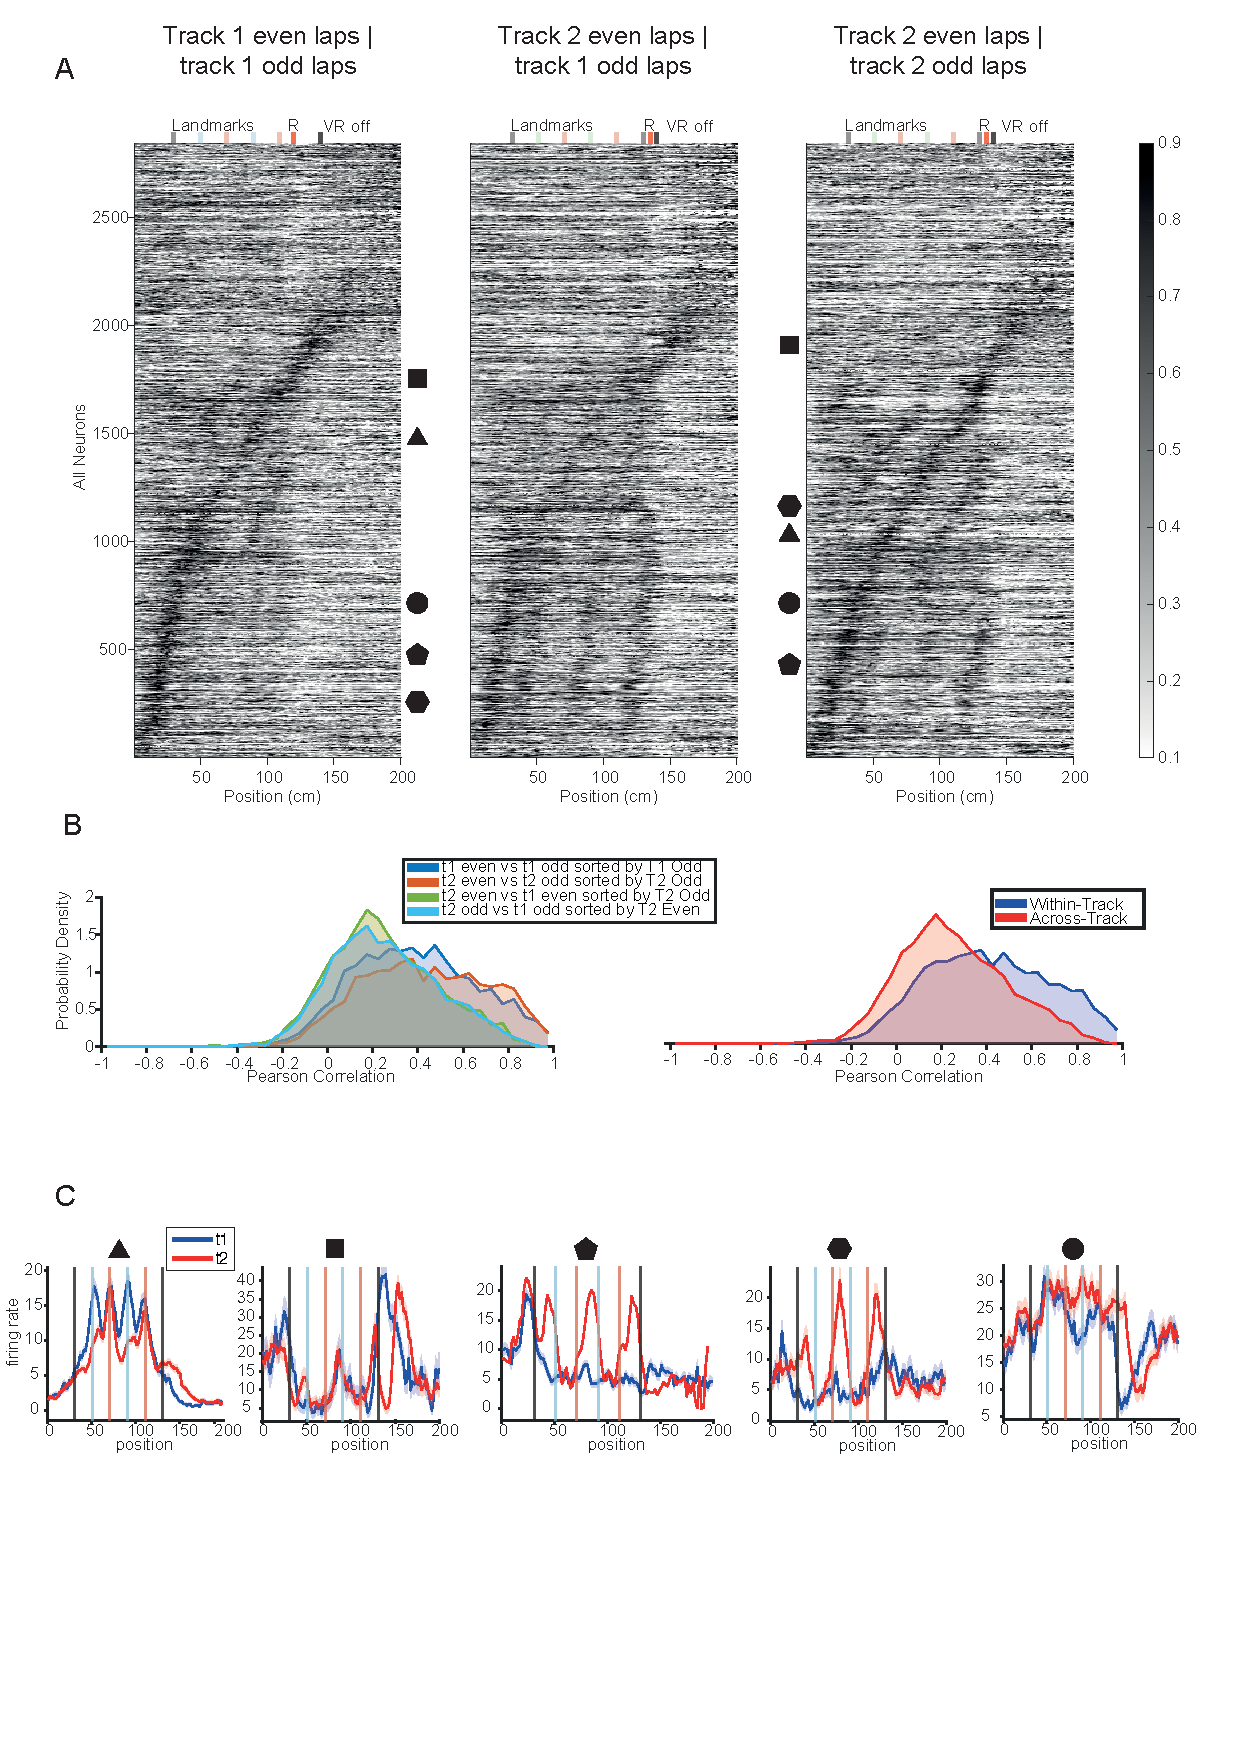
\includegraphics[width=1\linewidth]{figures//Chapter 5 MEC/fig1_MEC_spatial_tuning.pdf}
    \caption{MEC neurons are spatially tuned to positions in two environments and remap in the two environments.}
    \label{fig:MEC remapping}
\medskip
\small
\textbf{A)} Population maps of all MEC cells across sessions. From left to right is normalised average responses from either Track 1 or Track 2 even laps sorted by either peak locations in Track 1 odd laps or Track 2 odd laps. The position bin is extended outside of the VR during gray screen period between laps and the landmarks, rewards and VR off positions are labeled aobve the maps. \textbf{B)} Pearson correlation between two population maps in four pairs. Both panels are the same comparison but the one on the right merges pairs within track and pairs across track together. \textbf{C)} 5 example MEC neurons with high stability which show different degrees of spatial tuning and remapping. They are also labeled on panel \textbf{(A)}.
\end{figure}

\subsection{Speed Tuning}
In addition to spatial tuning, many MEC cells are tuned to the animal's running speed and some neurons have different speed tuning than linearly increasing speed cells in previous literature. The firing rate of the cell is binned by the animal's running speed and plotted in log scale in Fig 5.2A. A skewed gaussian curve is fitted to the responses. The peak of the best fit gaussian curve is what the cell is tuned to which is the preferred speed. The preferred speed is categorised into low-pass ( < 5 cm/s) , band-pass (5-30 cm/s), and high-pass ( > 30 cm/s). Many neurons have good fitting with this gaussian curve (Fig 5.2A) and there are cells tuned to all types of classifications: about 30\% not tuned, about 10\% low pass, about 5\% for each band of 5-20 band-pass, about 30\% for above 25 cm/s speeds. The gaussian curve fitting accounts for the linear increase in high speed preference cells which are likely speed cells found in previous literature. Beyond the classified cells, there are some cells classified as not tuned, for example the bottom right two example neurons in Fig 5.2 A, show more complex speed tuning where the middle one looks like an oscillation and the right-most one has high firing rate when stationary and firing rate increased after 20 cm/s speed. The gaussian curve fitting method works very well for many cells but can miss cells with complex tuning curve.
\begin{figure}
    \centering
    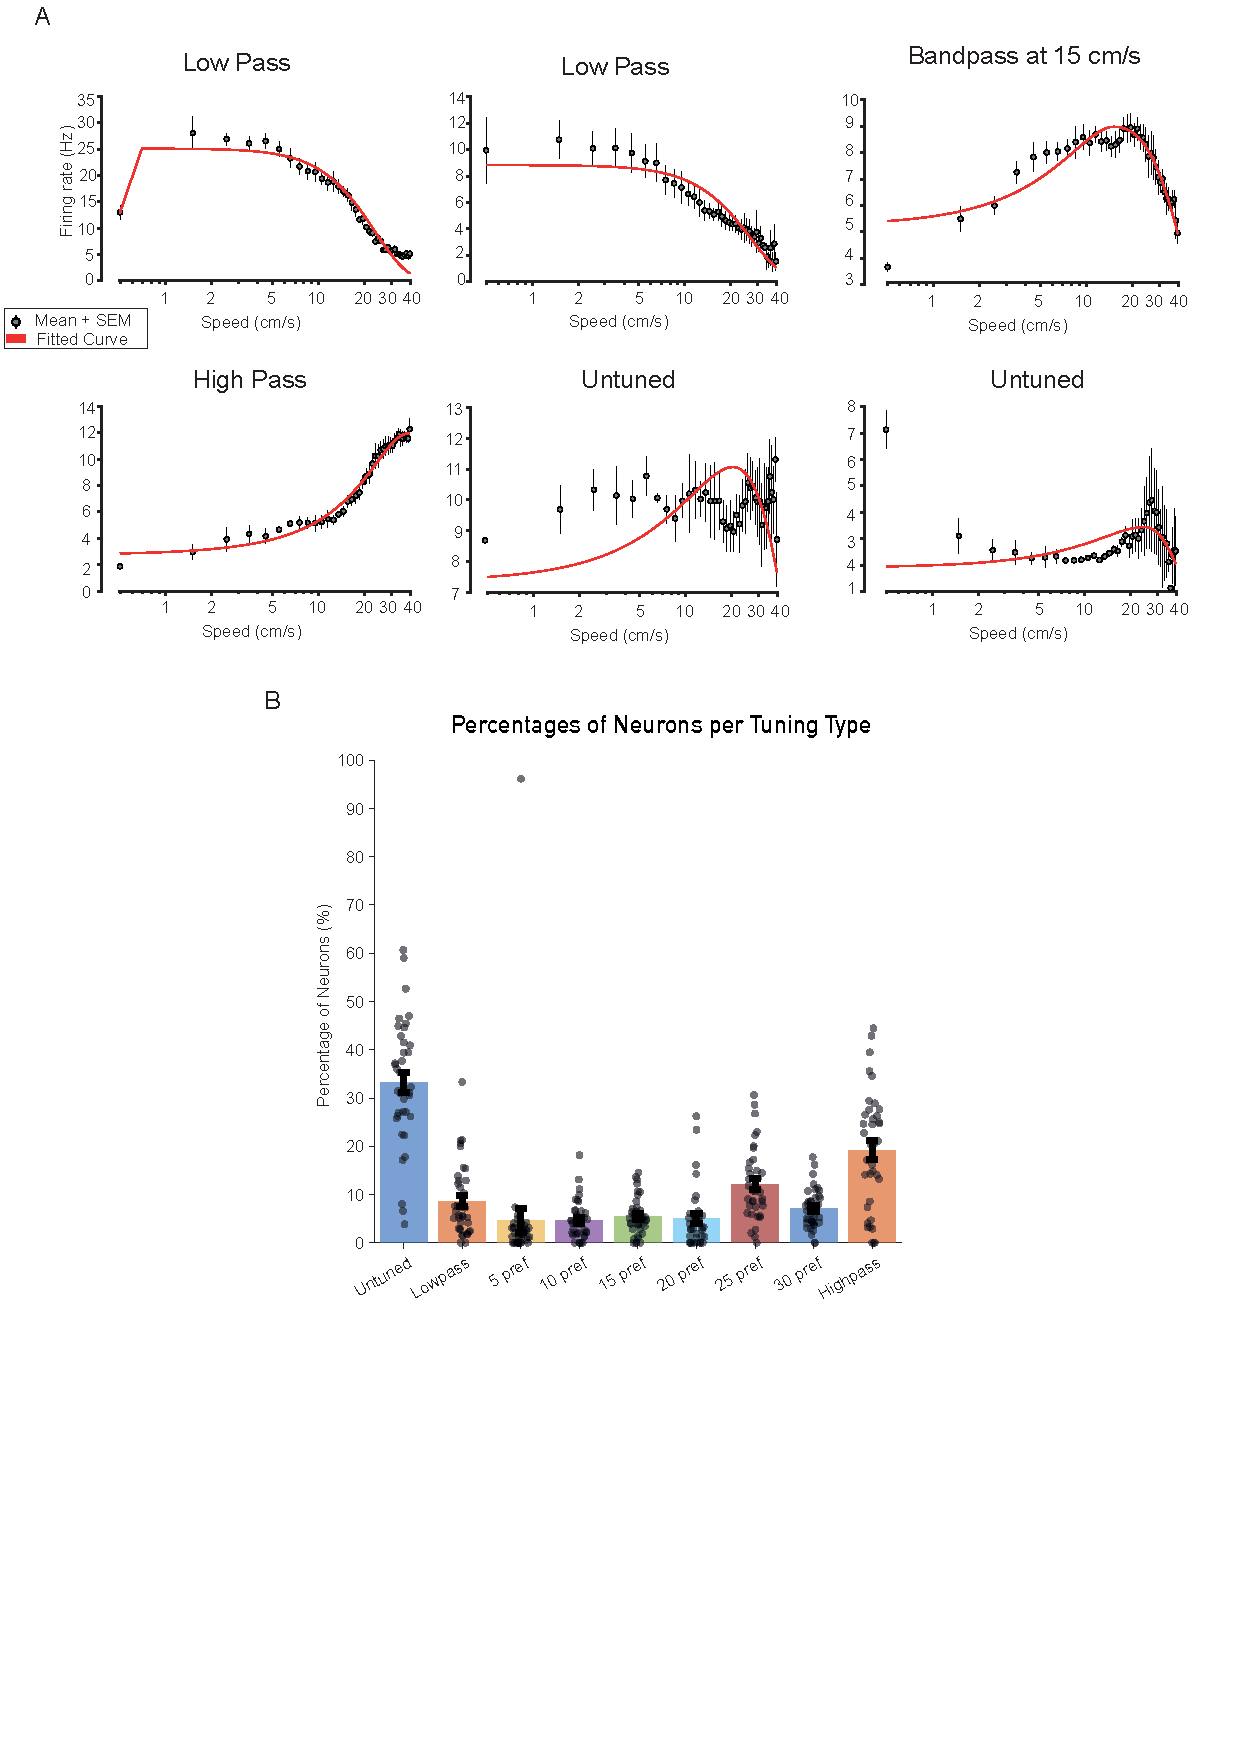
\includegraphics[width=1\linewidth]{figures//Chapter 5 MEC/fig2_speed_tuning.pdf}
    \caption{Speed Tuning in MEC}
    \label{fig:placeholder}
\medskip
\small
\textbf{A)} 6 example neurons' speed tuning. The x coordinate of animal's speed is in log scale. Each dot and its error bar is the neuron's firing rate at that speed. A fitted skewed gaussian curve in red is fitted to find the preferred speed of the neuron. \textbf{B)} Total percentages of neurons tuned to different speeds across sessions.
\end{figure}

\subsection{Multi-variate Tuning in MEC Cells}
MEC cells have subpopulations tuned to multiple variables and the interaction between variables can be additive or multiplicative at neuronal level. As described in previous V1 neuron characterisation chapter, a \(Speed \times Position \) binning method was used to compare speed impact on spatial binning. Here, the same method is used to understand the relationship between speed tuning and spatial tuning. In Fig 5.3A and Fig 5.3F, two example neurons with low-pass speed tuning and high-pass speed tuning respectively. In Fig 5.3A, the neuron has the low-pass speed tuning effect on the first spatial peak at the start of VR but the peaks at the end of VR around 135-160 cm have high firing rate at the peak positions whatever the animal's running speed is. In Fig 5.3F, the neuron has high-pass speed tuning effect on all the positional tuning across the VR from 30-150 cm in both tracks, but the neuron has no speed tuning at all in the rest including start of the VR and the gray screen period. In addition, the difference in position of the last peaks in track 1 and track 2 in Fig 5.3A and Fig 5.3B and the extra peak in track 2 of Fig 5.3F and Fig 5.3G can potentially be contributed by the reward responses as the reward zone is 115-125 cm in track 1 and 130-140 cm in track 2. In order to understand the multi-variate tuning in MEC cells, a generalised linear model is applied to the cells. The model has 5 cm bin spatial predictors for each track and speed predictors at 2.5 cm/s bins and a reward predictor at [0, 0.5]s time range. A poisson distrubtion log link function is used to connect all the predictors. For spatially relatively reliable neurons like Fig 5.3B and Fig 5.3G, the GLM predictions can mimic similar neural activities (Fig 5.3C, H) but the reward predictors contribute very little (Fig 5.3E, J). 
\begin{figure}
    \centering
    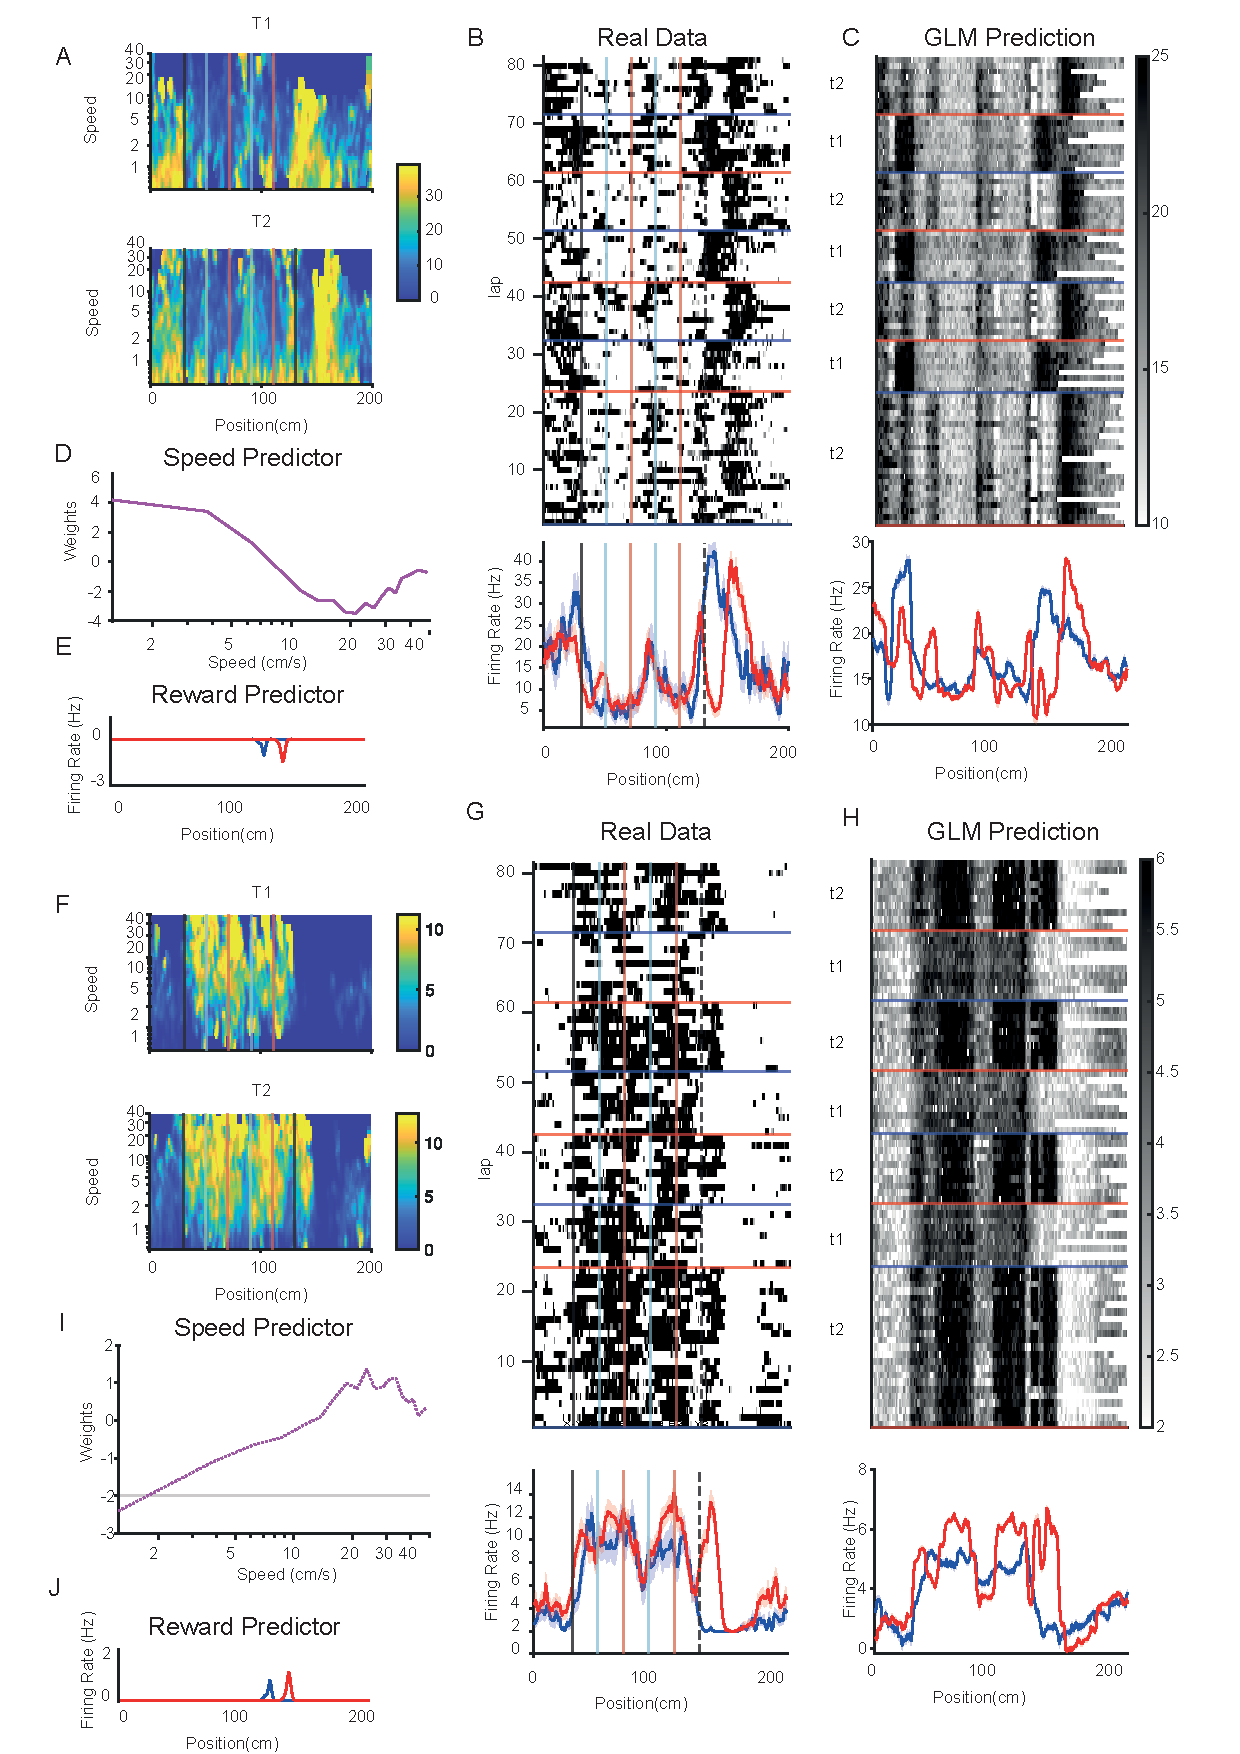
\includegraphics[width=1\linewidth]{figures//Chapter 5 MEC/fig3_multiple_navigational_variables.pdf}
    \caption{MEC Cells Tuned to Multiple Navigational Variables}
    
    \label{fig:placeholder}
\medskip
\small
In this figure, two example neurons are displayed and they separated by top and bottom rows. \textbf{A,F)} Firing rate is binned by \(Speed \times Position\) to show the impact of speed tuning on spatial tuning and top panel is track 1 and bottom panel is ttrack 2. \textbf{B, G)} The raster plots across the tracks of two example neurons and their PSTHs in the two tracks. \textbf{C, H)} Same as \textbf{(B,G)} but using predicted firing rates from a trained GLM model. \textbf{D, I)} Speed predictors' weights from the GLM model. \textbf{E, J)} Reward predictors' impact in the two tracks on the PSTH.
\end{figure}



\begin{figure}
    \centering
    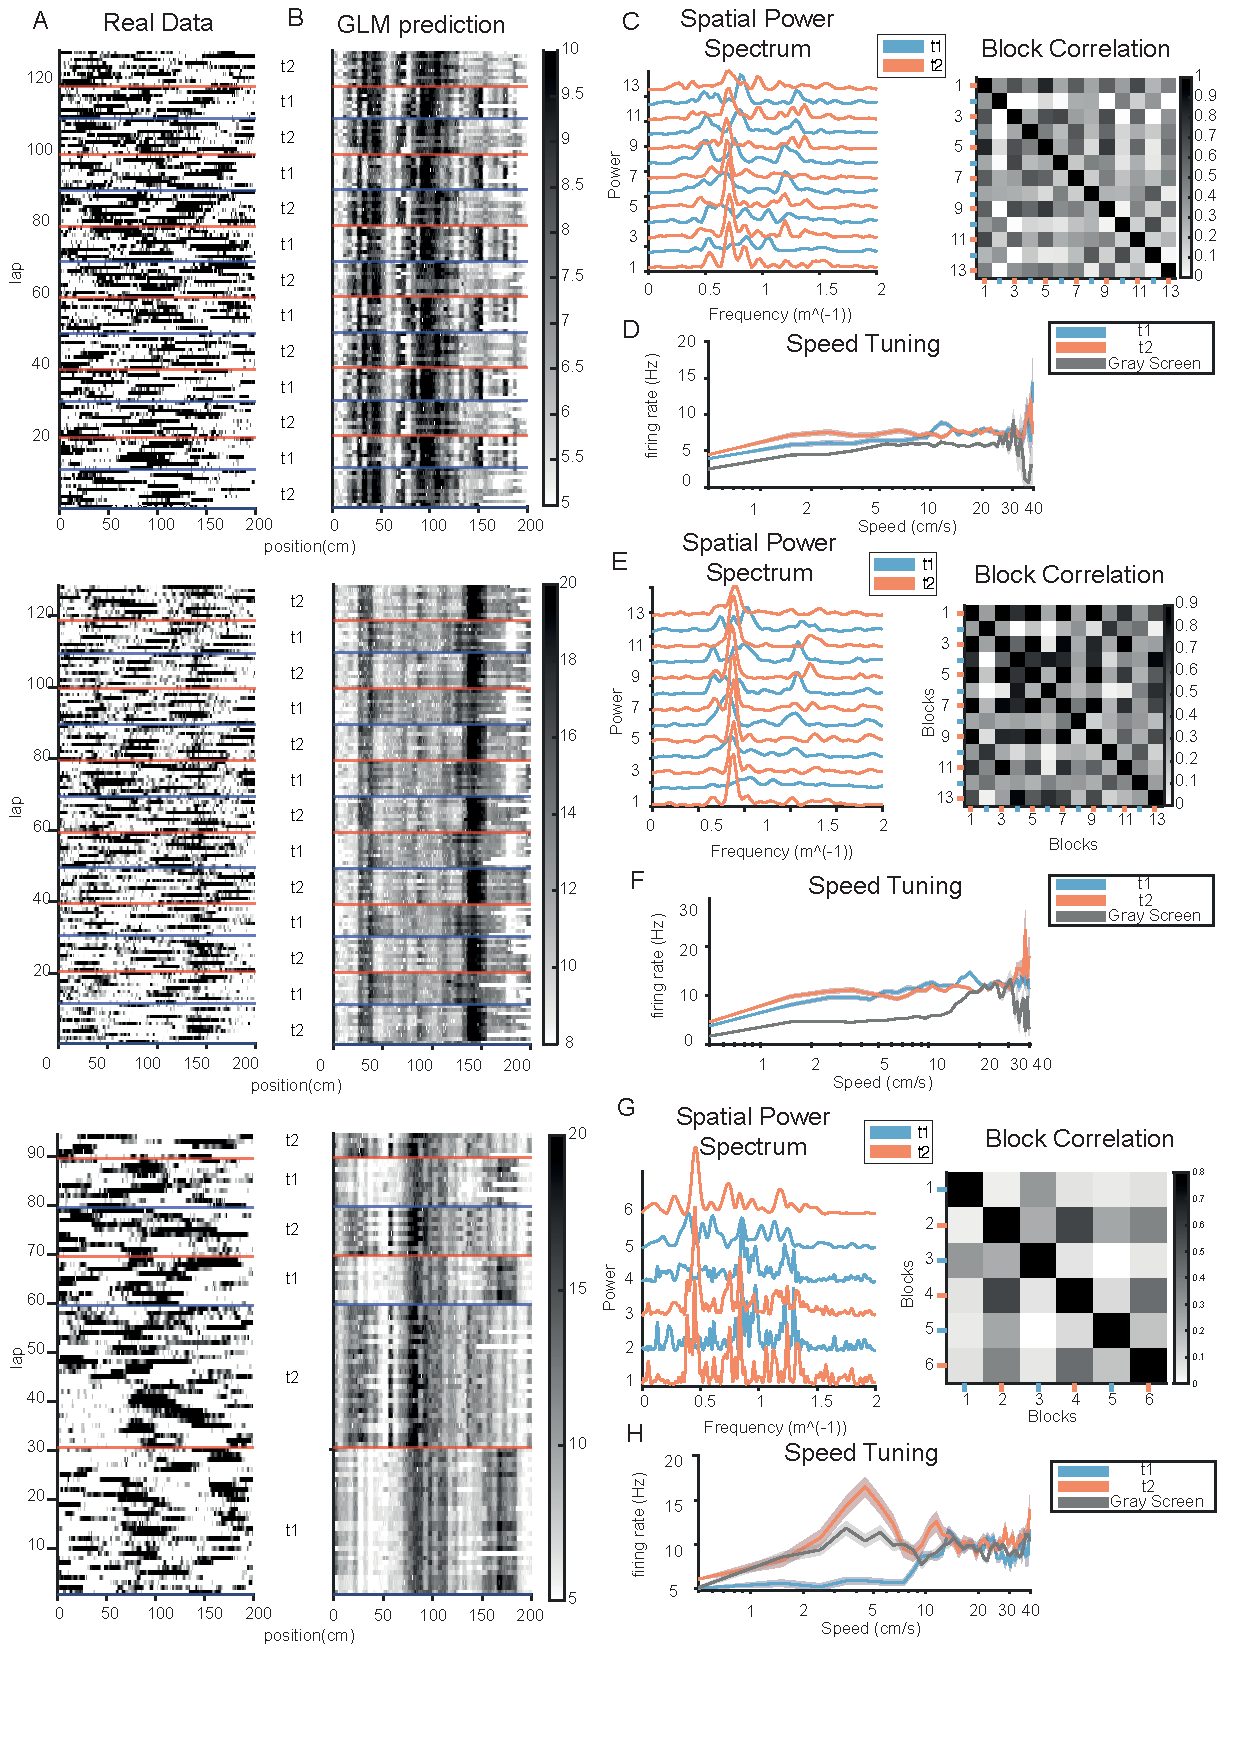
\includegraphics[width=1\linewidth]{figures//Chapter 5 MEC/fig4_periodic_firing.pdf}
    \caption{Periodic Firing Cells in MEC}
    \label{fig:placeholder}
    \medskip
\small
In this figure, three example neurons are displayed in three rows. \textbf{A, B)} show the real data against the GLM predictions same as in Fig 5.3. \textbf{C, E, G)} Spatial power spectrum is calculated from each block of laps in one track on the left panel and blue is track 1 and orange is track 2. The panel on the right is the correlations between the power spectrum across blocks. \textbf{D, F, H)} The speed tuning for the example neurons divided by track 1, track 2 and gray screen periods.
\end{figure}
\subsection{MEC Has a Subpopulation with Periodic Firing}
Some MEC cells do not show reliable spatial tuning throughout the two tracks but show periodic firing along positions. In some sessions, a group of MEC cells periodic firing at a range of frequencies along the VR (Fig 5.4A), and the GLM cannot capture this property and perform poorly (Fig 5.4A, B). In GLMs for these neurons, spatial predictors' weights are very low and they are unable to produce the trial-to-trial variability with position, speed and reward predictors (Fig 5.4B). In order to examine if these cells fire at fixed ranges of spatial frequencies, a spectrogram is estimated on each block of one track (Fig 5.4C, E, G) and the frequencies are restrained to within 2 meters. The two tracks are in blue and orange colours and the blocks from the same track have more similar power spectrum profiles but the peaks also drift over blocks (Fig 5.4C, E, G). For example, top example neuron has three peaks in all the track 1 blocks but the three peaks split further apart over blocks (Fig 5.4C). In order to compare the similarities between blocks and tracks, the correlations between blocks are shown in Fig 5.4C, E, G as well and they all exhibit a checkerboard like pattern which indicates that the spatial frequencies of the firing are different in the two tracks. In addition, there are local groups of blocks are more similar to each other no matter track. For example, blocks 4-6 are much more similar to each other in Fig 5.4G. Further to the periodic firing, some of these cells exhibit variations in speed tuning in the two tracks and gray screen period (Fig 5.4F, H), and especially bottom neuron in Fig 5.4H that the speed tunings of t1, t2, and gray screen are different from each other in the 2-10 cm/s band.



\section{Discussion}
In this chapter, MEC neurons show different degrees of remapping in the two tracks and subpopulations of them encode various navigational variables. In addition, some cells without reliable spatial responses at fixed locations can 'remap' at the level of their firing spatial frequency and potentially drift over blocks of switching between track 1 and track 2. In other studies, \cite{wen_one-shot_2024} also found that MEC cells drift a lot. But work in this thesis could not replicate their three-peak spatial power spectrum. This could be that this thesis's experiments do not have darkness running and the animal is trained for a long time in one environment. In this experimental design, the geometries of the two environments do not differ except the one additional landmark at the end in track 2 but the differences are mainly the contextual difference in the landmark patterns and reward zone location. In previous studies, grid cells only have realignment or rescaling when geometry of the environments is changed. In addition, changing landmarks' locations can also shift the grid cells immediately. Therefore, the MEC population in this experiment only has contextual changes and shift in response to the changes in at the end of VR. There are cells have more peaks in the novel environment and the frequency of the peaks is similar to the distance between sets of landmarks. This could indicate they are responses to the visual landmarks and MEC cells are more visual in novel environment but no conclusion at this stage. In \cite{wen_one-shot_2024}, they also found rapid peaks of responses to the landmarks when the mice were introduced to a novel environment with multiple landmarks. A control experiment would be swapping the novelty of the two tracks and also test if changing landmark visual patterns can change the firing patterns. In addition, many MEC cells are found to tune to multiple navigational variables in a multiplicative fashion agreeing to \cite{hardcastle_multiplexed_2017} and some visual cue and reward related peaks are additive (external cues). These findings imply that navigational variables are encoded in a multiplicative fashion, whereas external information variables are encoded in an additive fashion together with navigational variables. But such a claim requires further control experiments on how these firing patterns change when positions of landmarks and rewards are changed.However, most of the analyses are descriptive and more statistical tests are needed to show a complete analysis of the MEC population. 

